\section{Évaluation des extensions proposées}\label{sec:contribs:perf_eval}


Nous avons évalué les différentes améliorations proposées dans les sections~\ref{sec:openmp:langage} et~\ref{sec:openmp:runtime} sur les machines idchire et brunch, décrites en détails dans la section~\ref{sec:contribs:machines}.

Pendant le déroulement de cette thèse, les développeurs de Clang ont décidé d'adopter et d'intégrer officiellement le support exécutif d'Intel open source pour leur support d'OpenMP, et l'ont nommé libOMP.
Ce support exécutif dispose d'un support complet et robuste de la norme OpenMP~4.0, et utilise du vol de travail décentralisé (contrairement à libGOMP), avec également une découverte de la hiérarchie de la machine via hwloc.
La section suivante décrit l'implémentation de nos idées dans le support exécutif libOMP, la section~\ref{sec:contribs:perf_eval:logiciels} décrit le reste des logiciels que nous avons utilisés ; et enfin la section~\ref{sec:contribs:perf_eval:resultats} aborde point par point l'impact sur les performances des extensions proposées.

\subsection{Portage dans libOMP}\label{sec:contribs:perf_eval:libkomp}

Comme indiqué dans la section~\ref{sec:openmp:runtime:preliminary_results}, nous avions initialement implémenté nos idées dans XKaapi.
La structure de libOMP nous a semblé être une base favorable pour intégrer nos travaux et favoriser leur diffusion.
Cela nous permettait également d'ajouter des extensions directement dans Clang, tout en profitant au passage de la robustesse de son support d'OpenMP.
Nous avons donc étendu ce support exécutif avec la plupart des mécanismes présents dans XKaapi~: file de tâches non bornées (T.H.E), file de tâches hiérarchiques, et outils de génération de traces.
Nous l'avons renommé libKOMP.
Il s'agit là de la seconde version, bien différente de la version initiale publiée en 2012 par Broquedis et al.~\cite{Broquedis2012}.

\subsubsection{Extensions et options ajoutées}
\label{sec:contribs:perf_eval:portage_libkomp}

Le support exécutif libOMP fonctionne, pour les tâches, par vol de travail.
Chaque threads dispose d'une file de tâches, et les stratégies d'ordonnancement pour le placement et la sélection des files sont les suivantes, respectivement~: les tâches prêtes sont placées dans la file du thread courant~; lorsqu'un thread a besoin de voler du travail, il sélectionne aléatoirement une file de tâche d'un autre thread, s'il réussit un vol il reviendra voler cette victime la prochaine fois qu'il aura besoin de voler du travail.

Dans un premier temps, nous avons donc commencé par ajouter un ensemble de structures de données~: pour chaque nœud NUMA utilisé dans la \emph{team} OpenMP courante, nous avons ajouté une file de tâches, permettant ainsi d'exposer un second niveau de hiérarchie dans l'ordonnancement.
Nous avons également ajouté une file de tâche privée par thread et par nœud, pour implémenter la notion d'affinité stricte.

Dans un second temps, nous avons modifié les fonctions de placement des tâches prêtes et de sélection d'une victime à voler.
Nous avons directement implémenté la combinaison de stratégies qui obtenait le meilleur niveau de performances parmi celles présentées dans la section~\ref{sec:contrib:ws:heuristics}, à savoir~:
\begin{itemize}
  \item pour l'affinité entre une tâche et une donnée, le placement de la tâche est effectué selon la stratégie \emph{pNumaWLoc}, définie dans la section~\ref{sec:openmp:runtime:push}.
  \item la sélection d'une file de tâche à voler se fait hiérarchiquement, dans l'ordre indiqué par la stratégie \emph{sNumaProc}, défini dans la section~\ref{sec:openmp:runtime:select}.
\end{itemize}

Dans la suite des expériences, nous ferons référence à cette deuxième version de libKOMP en l'appelant tout simplement \emph{libKOMP}.


\subsection{Logiciels}\label{sec:contribs:perf_eval:logiciels}

Les logiciels utilisés pour nos expériences peuvent être divisé en trois catégories~:
\begin{itemize}
  \item Les applications, qui proviennent des KASTORS~;
  \item Les supports exécutifs~: libGOMP, libOMP, libKOMP~;
  \item Les bibliothèques externes~: BLAS, hwloc, et numactl.
\end{itemize}

Certaines applications et supports exécutifs utilisés ont dû subir quelques modifications afin d'incorporer les modifications d'OpenMP proposées.
Ces changements sont décrits ci-dessous.
Nous n'avons effectué aucune modification aux bibliothèques externes, mais il est important de faire un point dessus, étant donné qu'une partie des performances peut en dépendre.

\subsubsection{Applications utilisées}

Les applications utilisées pour ces expériences proviennent des KASTORS\footnote{https://gitlab.inria.fr/openmp/kastors, branche 'affinity'}.
Nous avons ajouté une clause \emph{affinity} dans certaines applications~: dans le cas des applications d'algèbre linéaire, les tâches de calculs dépendent d'un ou plusieurs blocs de données.
Compte tenu des premiers résultats que nous avons observé précédemment~\cite{Virouleau2016a}, nous avons estimé qu'ajouter une affinité entre chaque tâche et les données qu'elle écrit serait avantageux.
Dans le cas des applications de type stencil, nous avons ajouté une affinité vers un cœur précis pour les tâches successives.


\subsubsection{Supports exécutifs}


Nous avons pris comme base de comparaison les supports exécutifs fournis avec les compilateurs existants au moment de nos propositions.

\paragraph{GCC/libGOMP :} nous avons utilisé la version 7.2.0 comme référence, sans y apporter de modification.

\paragraph{Clang/libOMP :} nous avons utilisé la version 3.9. Bien que le support exécutif (libOMP) n'ait pas été modifié, le compilateur (Clang) a subit des modifications afin de supporter les clauses décrites dans la section~\ref{sec:openmp:langage}.

\subsubsection{Bibliothèques externes}

\paragraph{BLAS :} les applications d'algèbre linéaire des KASTORS dépendent de la bibliothèque BLAS.
Pour les expériences effectuées dans la section~\ref{sec:contribs:perf_eval:resultats}, nous avons utilisé la bibliothèque OpenBLAS~2.19 pour fournir les noyaux de calculs de base.


\paragraph{hwloc :} cette bibliothèque fournit les informations sur la hiérarchie de la machine, ainsi que des fonctions d'allocation de mémoire selon différentes politiques (voir section~\ref{sec:context:os:lib}). Nous avons utilisé la version 1.11.0.

\paragraph{numactl :} nous avons utilisé \emph{numactl} pour certaines courbes de référence. \emph{numactl} est fournie par libNUMA ; nous avons utilisé la version par défaut fourni par le fabricant de la machine.


\subsection{Résultats}\label{sec:contribs:perf_eval:resultats}

Les résultats obtenus sont illustrés ci-dessous, dans trois sections abordant des points importants~: la distribution des données, la prise en compte de la localité des données lors de l'exécution, et la possibilité de restreindre le vol de travail.

\subsubsection{Impact de la distribution des données}

\begin{figure}[ht]
  \centering
  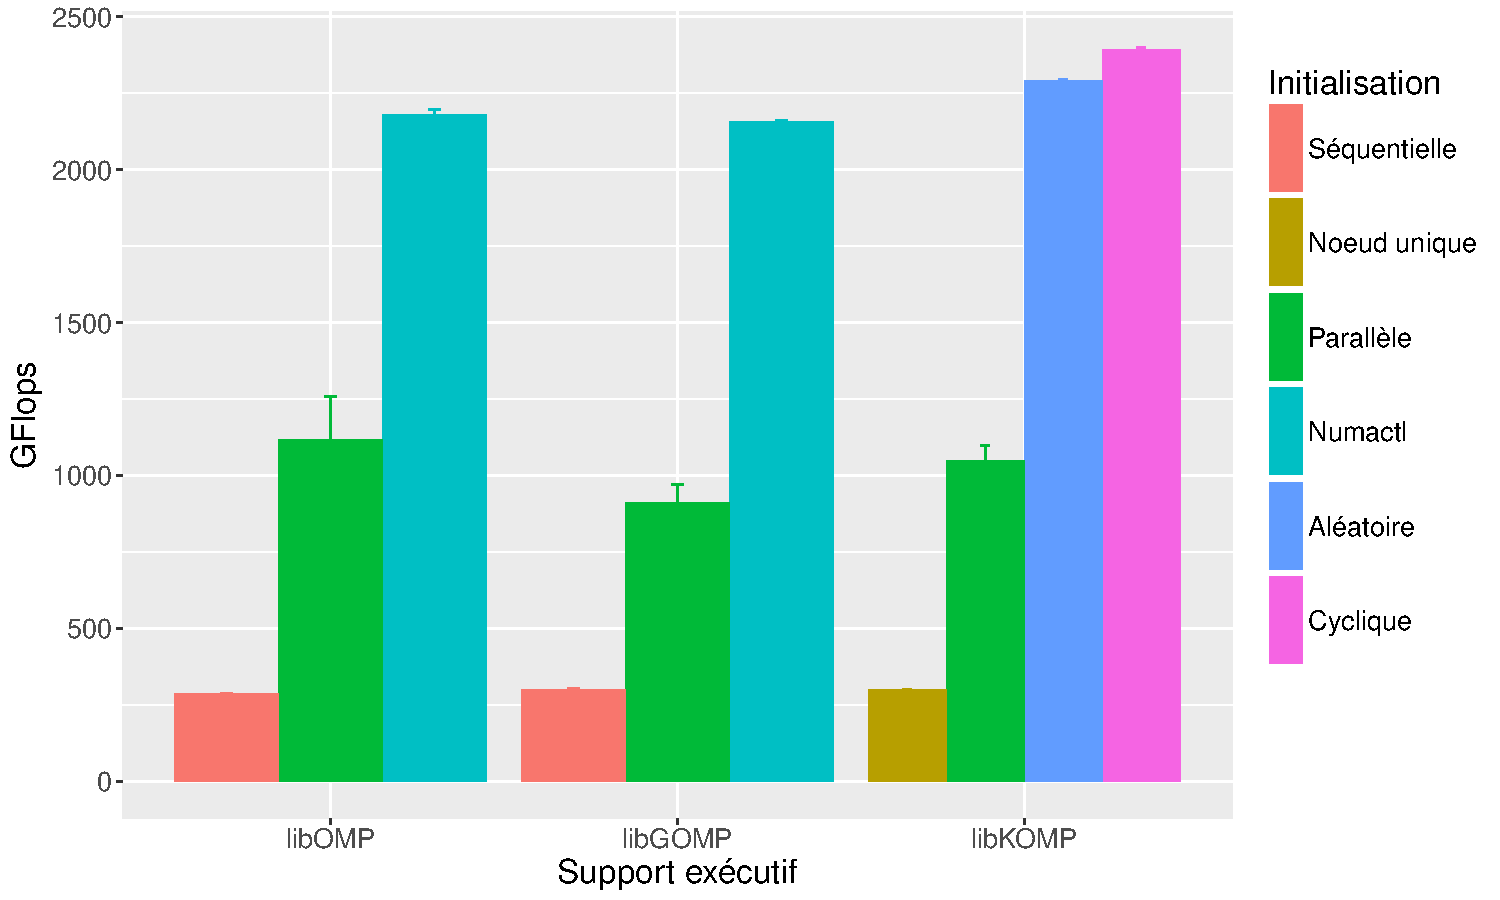
\includegraphics[width=\textwidth]{graph_distrib_data_idchire}
  \caption{Performances, sur les 192 cœurs d'idchire, des différentes stratégies pour Cholesky en fonction de la distribution de données. Taille de matrice~: 32768, taille de bloc~: 512}\label{fig:contribs:perf_eval:distrib-idchire}
\end{figure}


La figure~\ref{fig:contribs:perf_eval:distrib-idchire} montre un exemple représentatif du comportement de la factorisation de Cholesky par bloc, en fonction du support exécutif et du type de distribution de données. La taille de matrice utilisée est 32768, et la taille de bloc est 512, et la performance affichée est celle obtenue avec l'ensemble des 192 cœurs d'idchire.

La distribution \emph{Séquentielle} correspond à l'exécution du programme original.
La distribution \emph{Numactl} correspond à une distribution des pages des données effectuée de manière cyclique sur les nœuds de la machine à l'aide de \emph{numactl}.
Toutes les autres stratégies utilisent une initialisation parallèle dans laquelle chaque tâche est responsable de l'initialisation d'un bloc de données.

Parmi celles-ci, la distribution \emph{Non guidée} correspond à une distribution des tâches (et donc du placement des données, comme expliqué dans la section~\ref{sec:openmp:langage:init}) sur laquelle aucun contrôle n'a été effectué.
Néanmoins il y a une certaine distribution des tâches qui est naturellement effectuée~: compte tenu des tailles utilisées (64 blocs de largeur) et de la symétrie de la matrice, il y a 2080 blocs à initialiser et 24 nœuds sur la machine. En fonction de la rapidité d'initialisation du support exécutif, de la taille des files (si bornées), et de l'ordre dans lesquels les threads commencent à travailler, cette distribution non guidée peut varier.

La distribution \emph{Nœud unique} correspond au placement de toutes les tâches d'initialisation sur un seul nœud (ce qui revient à faire une initialisation séquentielle).
Les deux autres distributions, \emph{Cyclique} et \emph{Aléatoire} correspondent aux distributions que nous avons implémentées, et distribuent les tâche de manière cyclique ou aléatoire sur les nœuds de la machine.

La première chose à remarquer est que l'initialisation séquentielle de base (ou l'initialisation sur un nœud unique) propose sans surprise des performances désastreuses.

L'initialisation parallèle \emph{Non guidée} se distingue par sa variabilité~: les barres d'erreurs illustrent cette variabilité, due à l'ordre dans lesquels les threads viennent voler les tâches d'initialisation.

Au final l'utilisation de \emph{numactl} permet de contrebalancer les effets de l'initialisation séquentielle et d'atteindre des performances raisonnables.

La différence entre \emph{Numactl} et une distribution \emph{Aléatoire} peut être expliquée par le fait que \emph{numactl} distribue les \emph{pages} de manière aléatoire, alors qu'une distribution aléatoire des tâches d'initialisation distribue des \emph{blocs de données}, composés de plusieurs pages, ici 512 pages par bloc.

Ajouter une distribution de données spécifique assure que la distribution des tâches ne repose pas sur l'ordonnancement par défaut du support exécutif, et l'ordre parfois non contrôlé dans lequel les threads viennent voler du travail.
Bien que la différence ne soit que de quelques dizaines de GFlops, la distribution \emph{Cyclique} sur l'ensemble des nœuds NUMA semble être plus avantageuse que la distribution \emph{Aléatoire} sur l'ensemble des stratégies d'ordonnancement testé, et c'est celle qu'on a retenu pour les expériences des sections suivantes.


\subsubsection{Étude de l'impact de l'affinité}

Dans cette section, les résultats de libKOMP ont été obtenus avec une distribution \emph{Cyclique} et avec une combinaison de stratégies prenant en compte l'affinité et les deux niveaux de hiérarchie des machines.
Nous avons étudié l'impact de l'affinité sous plusieurs angles~:

\paragraph{Performances brutes}

\begin{figure}[h!]
  \centering
  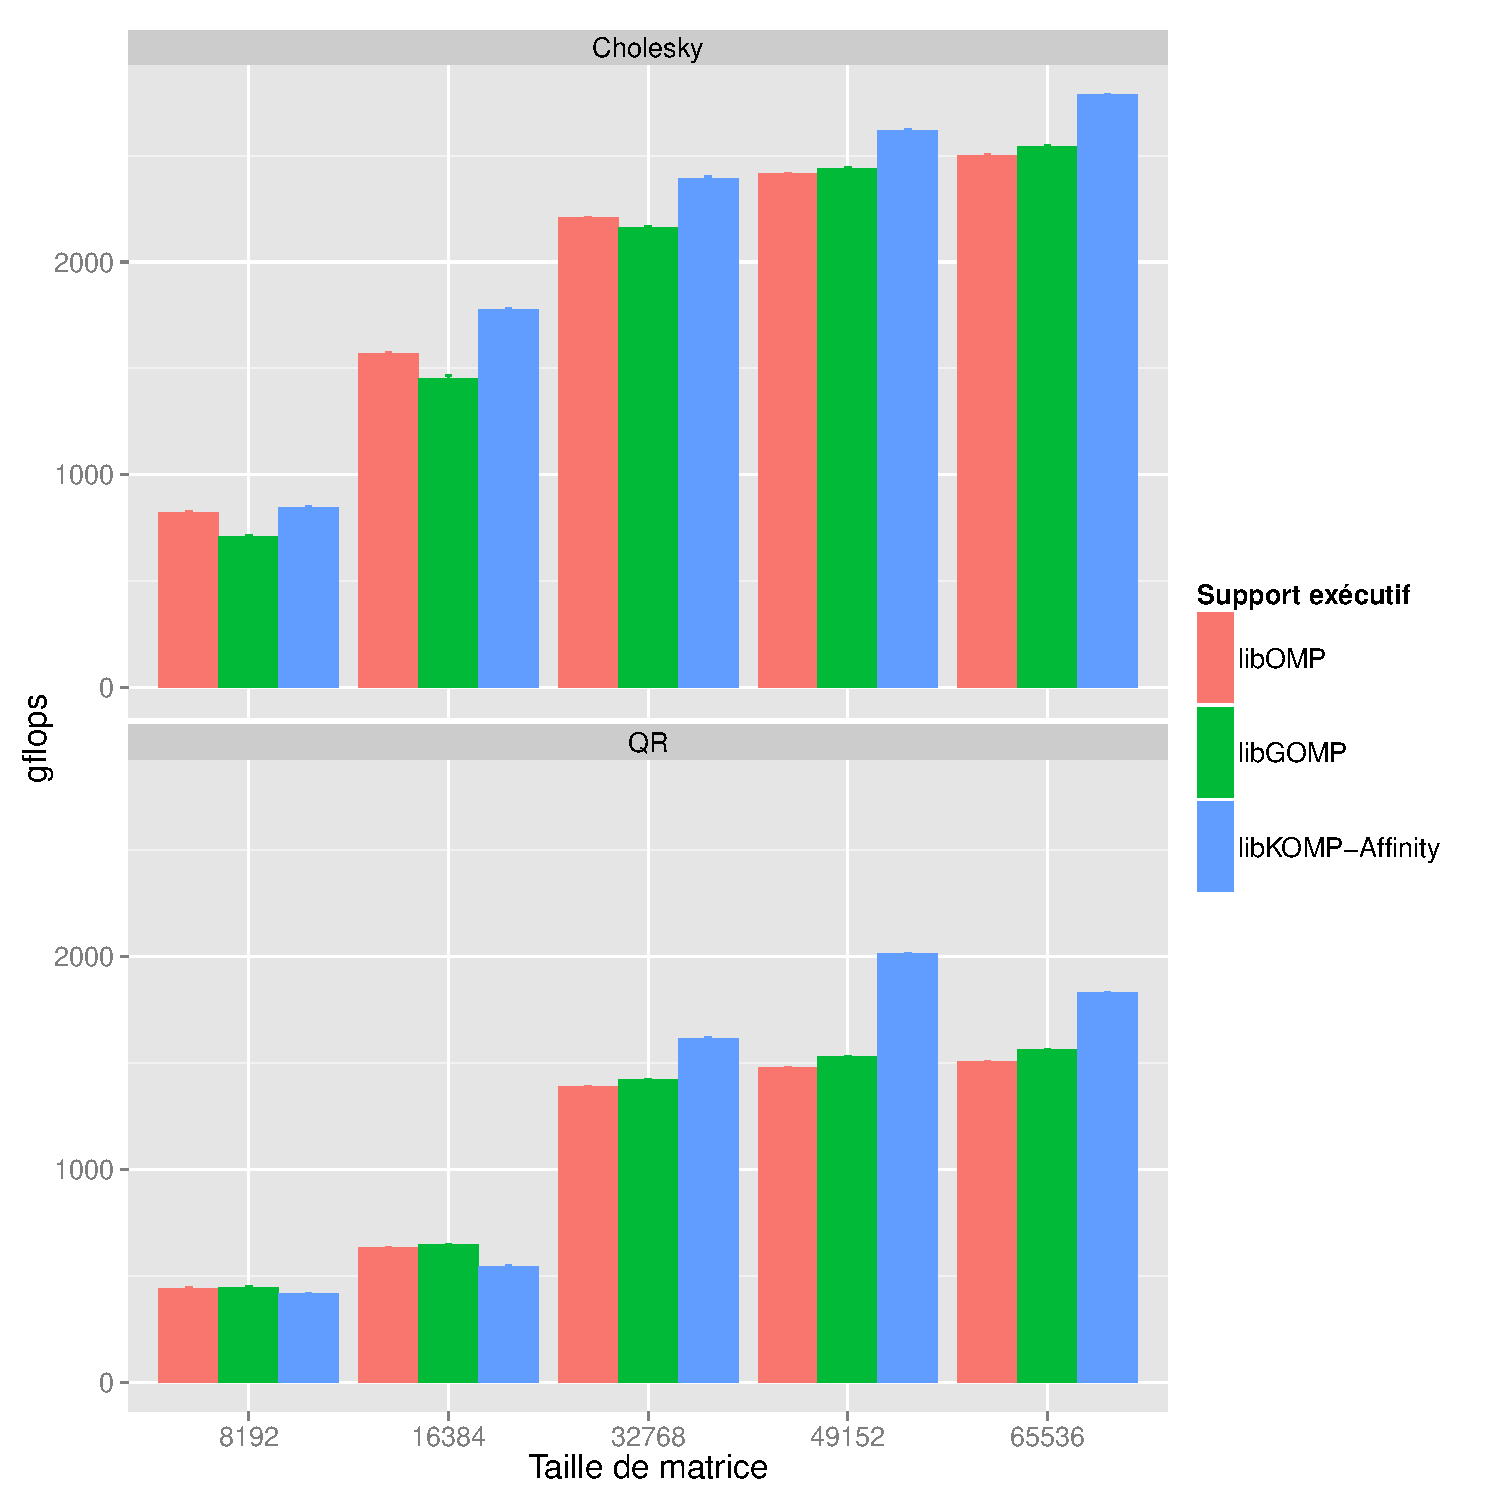
\includegraphics[width=\textwidth]{graph_details_qr_cholesky_idchire}
  \caption{Comparaison des supports exécutifs sur Cholesky et QR sur idchire, en fonction de la taille de matrice (tailles de bloc données dans le tableau~\ref{tab:perf_eval:blocksizes})}\label{fig:contribs:perf_eval:eval-qr-cholesky}
\end{figure}

Pour avoir un aperçu général des stratégies que nous avons évaluées sur les factorisations Cholesky et QR, avec des tailles de matrice variant entre 16384 et 65536~; les tailles de blocs correspondantes sont détaillées dans le tableau~\ref{tab:perf_eval:blocksizes}.

\begin{table}[h!]
\def\arraystretch{1.5}
\centering
\begin{tabular}{|c|c|c|c|c|c|}\hline
  Taille de matrice & 8192 & 16384 & 32768 & 49152 & 65536 \\\hline
  Taille de bloc & 256 & 256 & 512 & 512 & 512 \\\hline
\end{tabular}
\caption{Tableau de correspondance entre taille de matrice et taille de bloc}\label{tab:perf_eval:blocksizes}
\end{table}

\begin{figure}[h!]
  \centering
  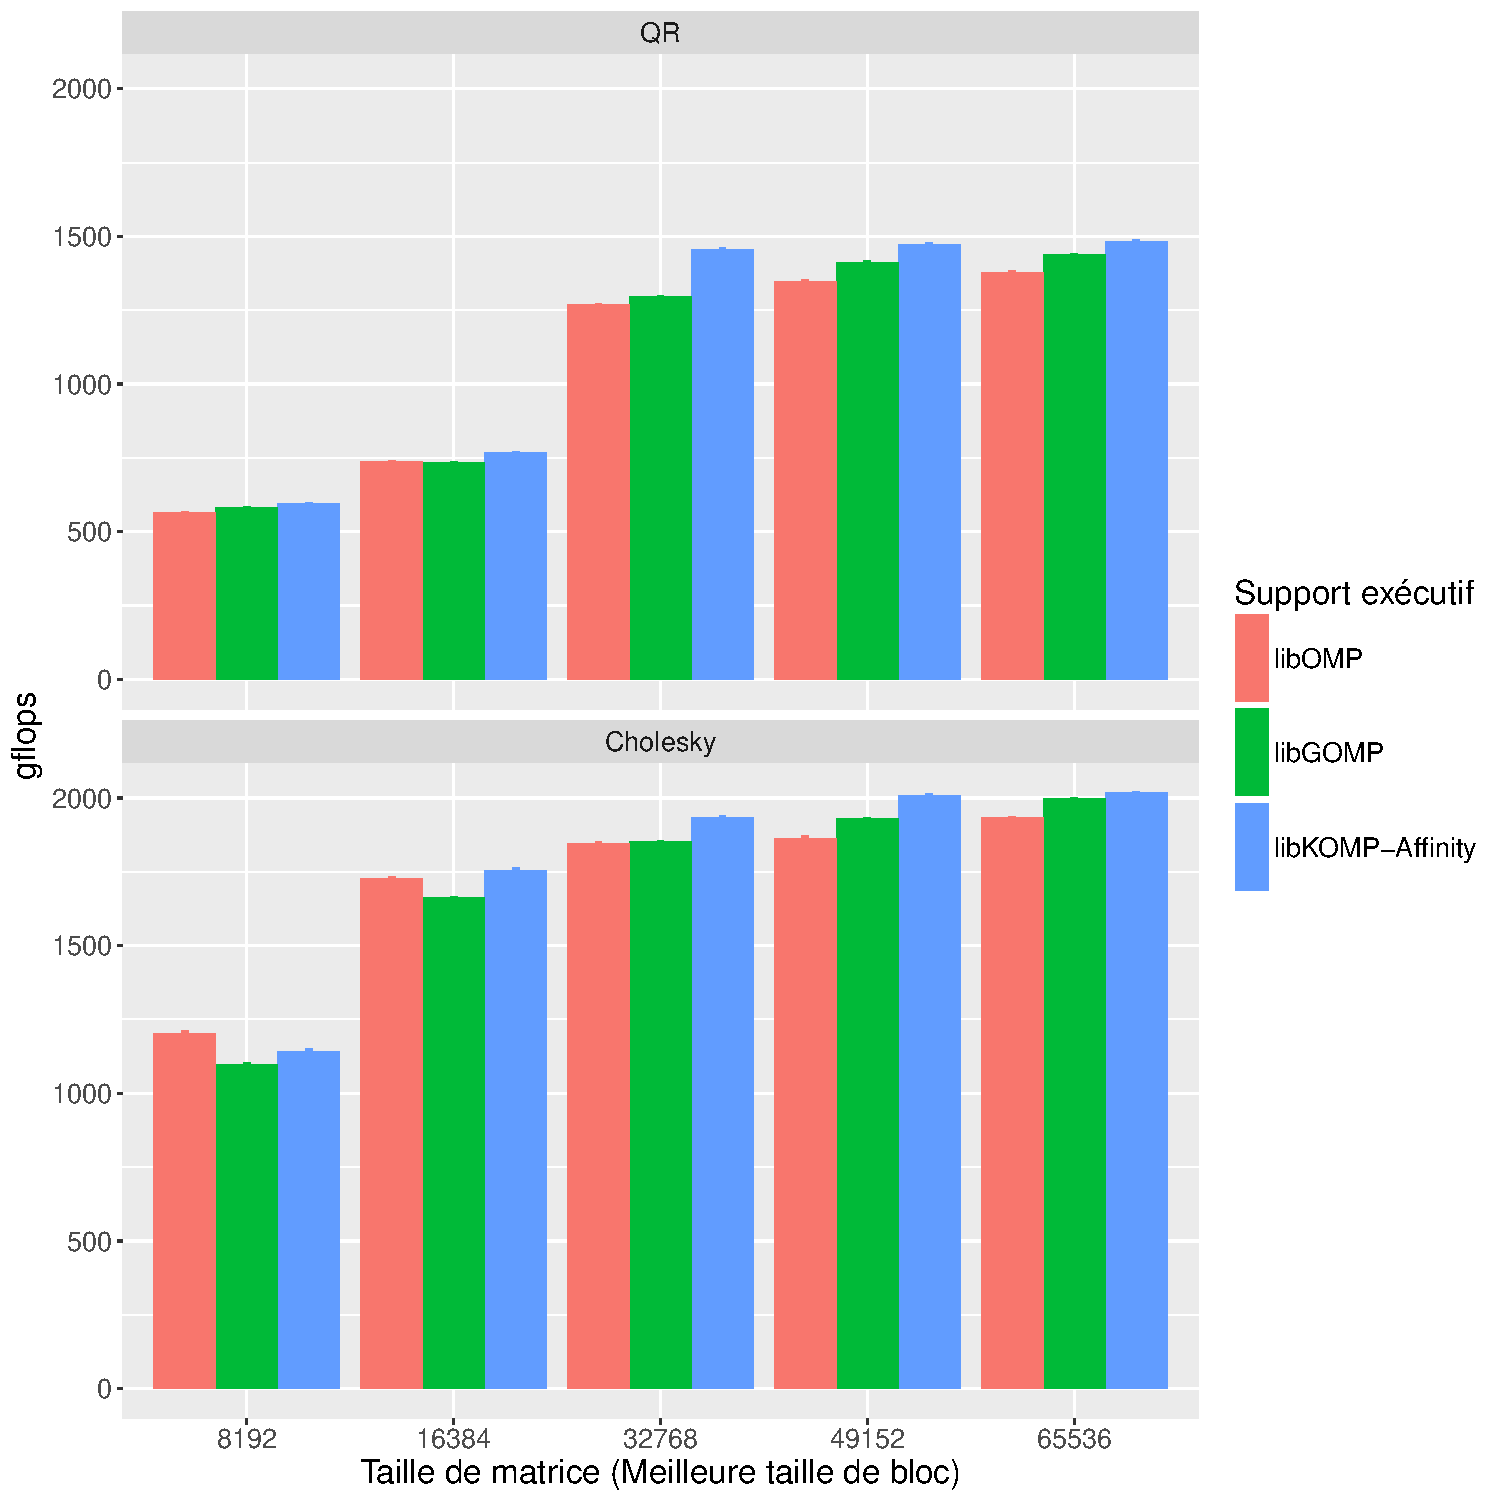
\includegraphics[width=\textwidth]{graph_details_qr_cholesky_brunch}
  \caption{Comparaison des supports exécutifs sur Cholesky et QR sur brunch, en fonction de la taille de matrice (tailles de bloc données dans le tableau~\ref{tab:perf_eval:blocksizes})}\label{fig:contribs:perf_eval:eval-qr-cholesky-brunch}
\end{figure}

La figure~\ref{fig:contribs:perf_eval:eval-qr-cholesky} montre les résultats obtenus sur idchire, et la figure~\ref{fig:contribs:perf_eval:eval-qr-cholesky-brunch} montre les résultats obtenus sur brunch.


Les machines brunch et idchire ont un facteur NUMA différent~: le coût d'accès à la mémoire distante par rapport à la mémoire locale est beaucoup plus important sur idchire que sur brunch.
Malgré cela, l'impact de l'affinité est bien visible sur les deux machines, même s'il est proportionnellement plus important sur idchire.

On peut observer que pour les faibles tailles de matrices, l'intérêt de l'affinité semble limité.
Plutôt que de regarder la taille de matrice, il faut en fait regarder la taille de bloc pour trouver l'explication de la différence~: pour les tailles de matrice 8192 et 16384 la taille de bloc est de 256, pour les autres elle de 512.
Les tailles de blocs induisent une différence claire vis à vis du cache L3~: dans le cas des blocs de taille 256 l'ensemble des données de calcul pour chaque noyau de l'application tient dans le cache L3, ce qui n'est pas le cas pour les blocs de taille 512.
Compte tenu des résultats montrés dans la section~\ref{sec:contribs:apps:cholesky:locality}, qui ont montré la dégradation très importante des performances lorsque les données ne tenant pas dans le cache sont à distance, il est donc logique d'observer l'amélioration significative des performances pour de grande tailles de blocs (nécessaires pour les grandes tailles de matrices), et une différence relativement faible concernant les tailles de blocs plus petites.


\paragraph{Évolution en fonction du nombre de cœurs}

La figure~\ref{fig:contribs:perf_eval:eval-cholesky-idchire} illustre l'évolution de l'impact de l'affinité en fonction du nombre de cœurs et de la taille de matrice sur idchire.


\begin{figure}[ht]
  \centering
  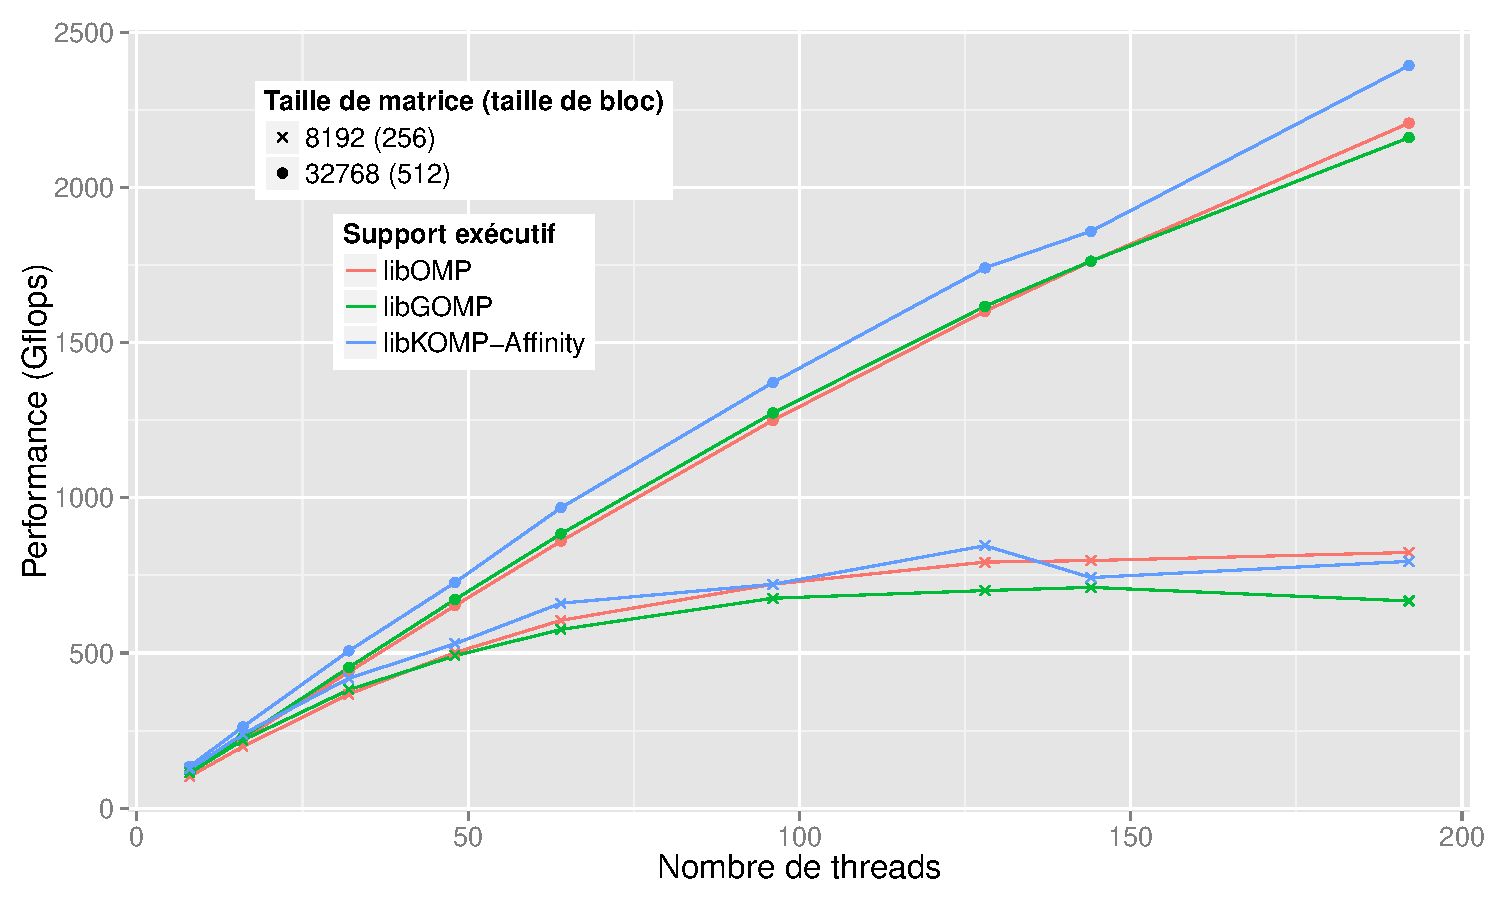
\includegraphics[width=\textwidth]{graph_all_cholesky_idchire}
  \caption{Performance en fonction du nombre de cœurs et de la taille de matrice sur idchire}\label{fig:contribs:perf_eval:eval-cholesky-idchire}
\end{figure}

Comme pour les expériences précédentes, les tailles de blocs correspondantes sont 256 pour la taille 8192, et 512 pour la taille 32768.
Les deux tailles de matrice choisies représentent les deux situations décrites précédemment~: dans un cas les données des noyaux de Cholesky tiennent dans le cache L3, dans l'autre non.
Dans le cas d'une petite taille de bloc on peut constater que la courbe de libKOMP se situe entre libOMP et libGOMP, ne donnant donc aucun résultat concluant, voire même étant coûteux par rapport à un simple vol de travail aléatoire comme dans libOMP !
Pour une grosse taille de bloc en revanche c'est clair et net~: après avoir suivi le même départ, les courbes divergent. Les supports exécutif libOMP et libGOMP affichent les même performances, tandis que l'affinité offre un net gain.

\begin{figure}[t!]
  \centering
  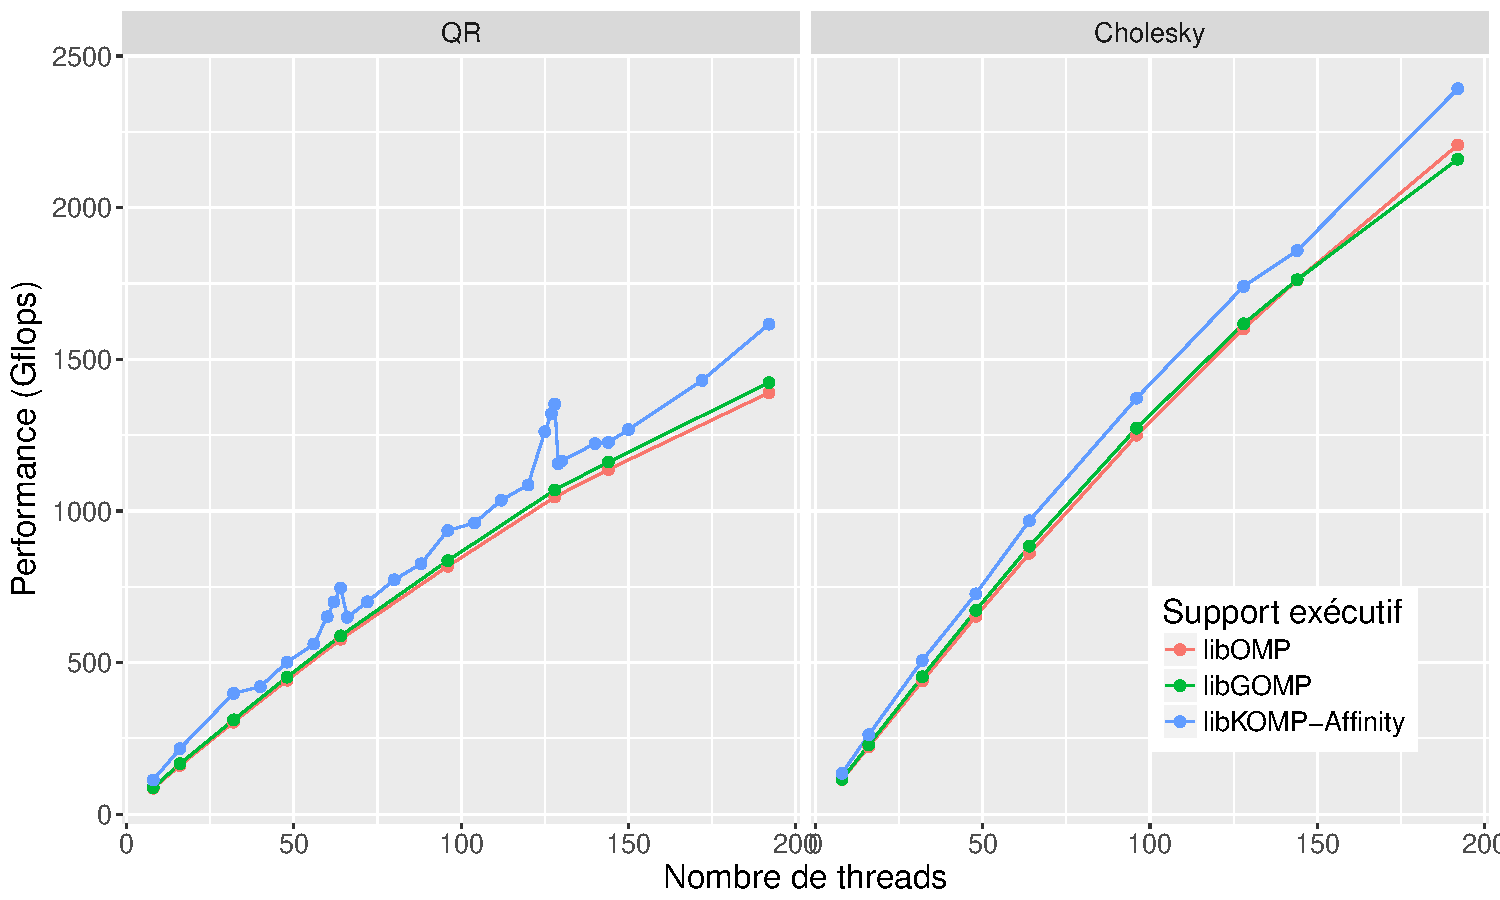
\includegraphics[width=\textwidth]{graph_qr_cholesky_vs_threads}
  \caption{Performance de Cholesky et QR en fonction du nombre de cœurs sur idchire. Taille de matrice~: 32768, taille de bloc~: 512}\label{fig:contribs:perf_eval:eval-qr-cholesky-idchire}
\end{figure}
\begin{figure}[h!]
  \centering
  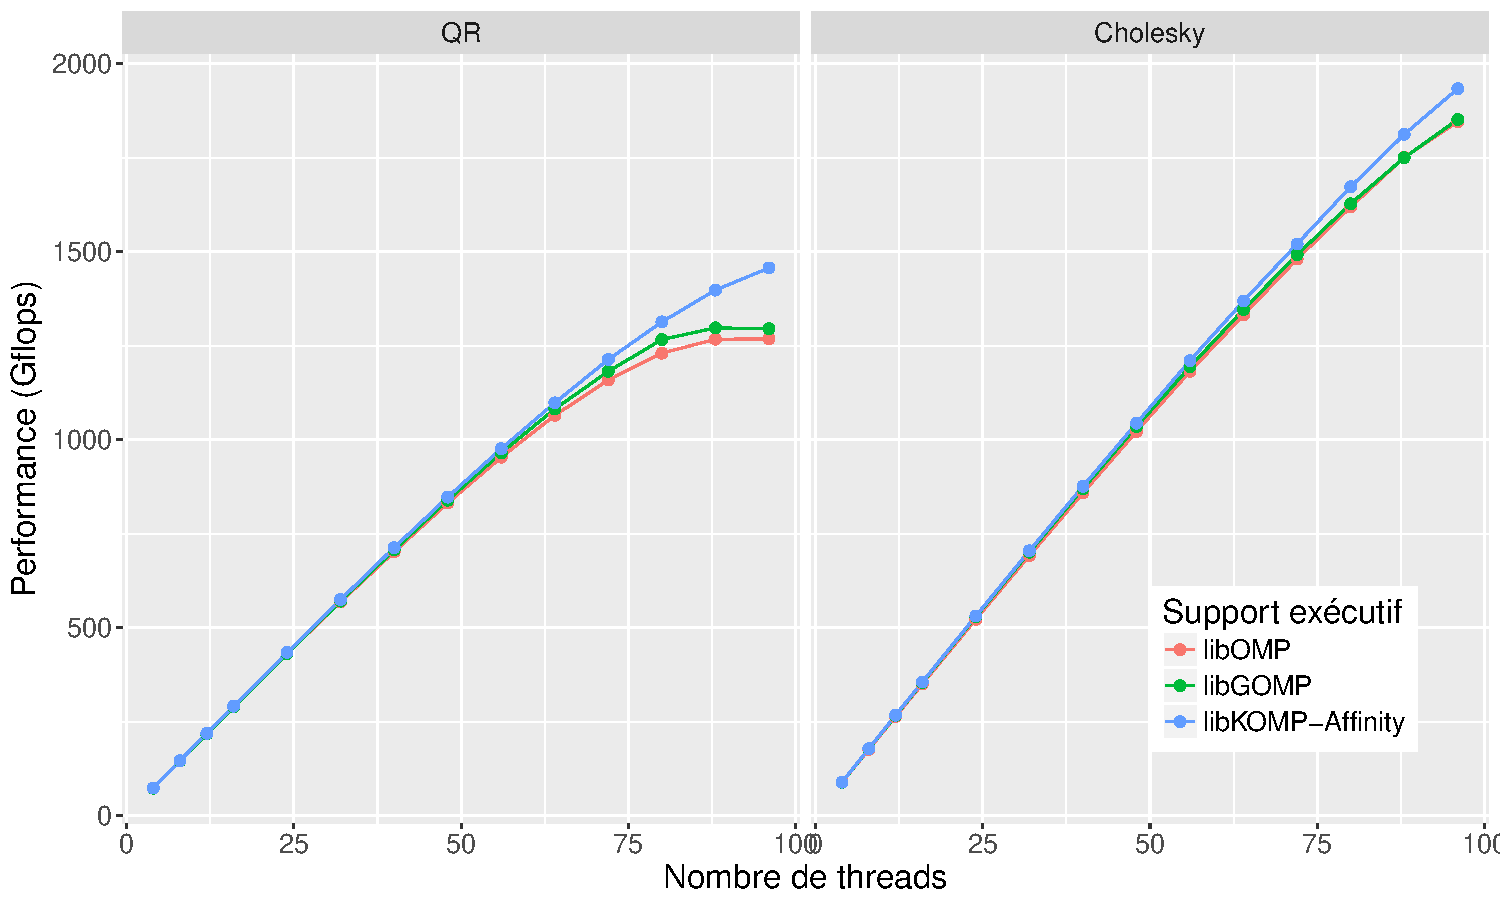
\includegraphics[width=\textwidth]{graph_qr_cholesky_vs_threads_brunch}
  \caption{Performance de Cholesky et QR en fonction du nombre de cœurs sur brunch. Taille de matrice~: 32768, taille de bloc~: 512}\label{fig:contribs:perf_eval:eval-cores-qr-cholesky-brunch}
\end{figure}

Les figures~\ref{fig:contribs:perf_eval:eval-qr-cholesky-idchire} et~\ref{fig:contribs:perf_eval:eval-cores-qr-cholesky-brunch} montrent les résultats des factorisations Cholesky et QR (taille de matrice 32768, taille de bloc 512) en fonction du nombre de threads sur idchire et brunch, respectivement.
Comparer les mêmes instances sur les deux machines donne des résultats intéressants~: leurs caractéristiques ne changent pas l'allure général des courbes, en revanche le faible facteur NUMA de brunch fait bien sentir que l'affinité n'est rentable que lorsque la machine est chargée à partir d'un seuil élevé (environ 75\%).
Alors que sur idchire la différence se voit dès une trentaine de cœur (qui correspond d'ailleurs à 4 nœuds NUMA).

En faisant ces expériences nous avons constaté un comportement assez atypique de QR avec l'affinité~: il y a 3 petits pics de performances à 32, 64, et 128 cœurs (soit 4, 8, et 16 nœud NUMA) !
Nous n'avons pas pu faire une étude aussi approfondie de QR que de Cholesky, il est donc dur d'expliquer ce comportement qui doit être dû à certaines caractéristiques de l'application.

%mais ici on peut penser que la distribution des données est responsable de ces pics. La distribution utilisée est cyclique, et sur un nombre de nœud NUMA en puissance de 2 cela doit fournir des propriétés favorables à l'application.



\subsubsection{Affinité stricte}

La section~\ref{sec:openmp:langage:affinity} introduit la clause affinité en précisant que l'utilisateur peut spécifier une affinité \emph{stricte}, restreignant ainsi les décisions d'ordonnancement du support exécutif.
Cette fonctionnalité n'a pas été utilisée pour les applications d'algèbre linéaire, car dans les cas que nous avons étudiés il était plus rentable de payer le coût de transfert des blocs de données plutôt que de se priver du parallélisme disponible.
Ce n'est évidemment pas le cas pour toutes les applications, et les applications stencil, comme Jacobi, peuvent grandement bénéficier d'une restriction d'affinité aux ressources proches, du fait de leur faible intensité opérationnelle (dans le cas de Jacobi, elle est en $O(1)$).

\begin{figure}[ht]
  \centering
  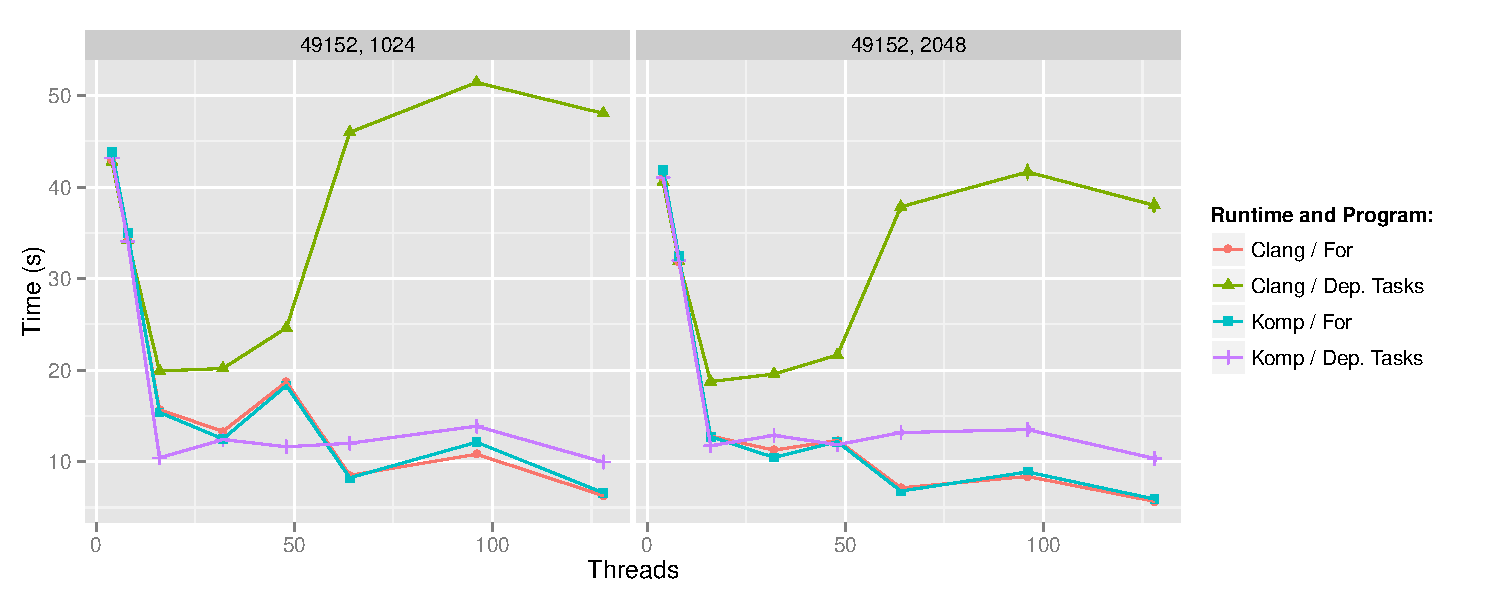
\includegraphics[width=\textwidth]{jacobi_scale_iomp_komp}
  \caption{Performances de Jacobi en fonction de la version et du support exécutif, avec une taille de matrice de 49152, sur idchire}\label{fig:contribs:perf_eval:eval-jacobi}
\end{figure}

La figure~\ref{fig:contribs:perf_eval:eval-jacobi} montre les performances de Jacobi sur deux tailles de blocs différentes.
Les mesures avec l'affinité ont été effectuées avant le portage dans libOMP, et le support exécutif sous-jacent est donc XKaapi.
La version à base d'OpenMP |for| utilise un ordonnancement statique, sans contrôle particulier sur la distribution des données.
Les versions à base de tâches avec dépendances n'utilisent aucun contrôle sur le placement des tâches ou des données.
Pour la version avec affinité, une distribution de données a été rajoutée dans l'application, avec également une affinité stricte suivant cette distribution de données sur les itérations successives.
Cette distribution affecte les blocs de données sur une grille la plus carrée possible en fonction des nœuds utilisés.
L'affinité stricte ajoutée permet de garantir la réutilisation des données présentes dans le cache L2 (point critique pour cette application), et éviter des migrations de tâches inappropriées, ce qui est d'autant plus important que l'intensité opérationnelle est faible.
Les performances obtenues avec les versions à base de boucles sont faibles comparativement aux résultats de l'affinité, néanmoins cela vient du fait qu'il n'y a pas eu d'effort particulier de fait pour que le découpage des itérations correspondent à celui des distributions des données.
Les performances des deux versions devraient théoriquement être équivalentes~: l'affinité stricte est là pour restreindre la portée du vol de travail qui dégradait les performances, phénomène qui ne devrait pas être présent dans une version à base de boucles.
